\documentclass[a4paper, 12pt]{article}
\usepackage[utf8]{inputenc}

\usepackage[a4paper,top=1.3cm,bottom=2cm,left=1.5cm,right=1.5cm,marginparwidth=0.75cm]{geometry}
\usepackage{cmap}				
\usepackage{mathtext} 				
\usepackage[T2A]{fontenc}			
\usepackage[utf8]{inputenc}			
\usepackage[english,russian]{babel}	
\usepackage{multirow}
\usepackage{mathtools}
\mathtoolsset{showonlyrefs=true}

\usepackage{graphicx}
\usepackage{wrapfig}
\usepackage{tabularx}
\usepackage{caption}

\title{2.1.3-theory}
\author{Влад Черниенко}
\date{March 2022}


\begin{document}

    \begin{titlepage}
    
        \begin{center}
            {\large МОСКОВСКИЙ ФИЗИКО-ТЕХНИЧЕСКИЙ ИНСТИТУТ (НАЦИОНАЛЬНЫЙ ИССЛЕДОВАТЕЛЬСКИЙ УНИВЕРСИТЕТ)}
        \end{center}
        \begin{center}
            {\large Физтех-школа радиотехники и компьютерных технологий}
        \end{center}
        
        \vspace{4.5cm}
        
        {\huge
            \begin{center}
                {\bf Лабораторная работа 3.2.6} \\
                Изучение гальванометра
            \end{center}
        }
        
        \vspace{12cm}
        
        \begin{flushright}
            {\LARGE Автор: \\ Черниенко Владислав Антонович \\ \vspace{0.2cm} Группа Б01-110}
        \end{flushright}
        
    \end{titlepage}
    
    
    \noindent {\bf Цель работы:} изучение работы высокочувствительного зеркального гальванометра магнитоэлектрической системы в режимах измерения постоянного тока и электрического заряда. \\
    
    \noindent {\bf В работе используются:} зеркальный гальванометр с осветителем и шкалой, источник постоянного напряжения, делитель напряжения, магазин сопротивлений, эталонный конденсатор, вольтметр, переключатель, ключи, линейка. \\
    
    \begin{flushleft}
        {\Large {\bf Теоретические сведения}}
    \end{flushleft}
    
    \textit{Баллистическим гальванометром} называют электроизмерительный прибор магнитоэлектрической системы, отличающийся высокой чувствительностью к току и сравнительно большим периодом колебаний подвижной системы (рамки). \\
    
    \noindent {\bf A. Определение динамической постоянной гальванометра\\Экспериментальная установка} \vspace{0.1cm}
    
    Схема для исследования гальванометра в стационарном режиме представлена на рис. \ref{pic1}. Постоянное напряжение $U$ снимается с блока питания и измеряется вольтметром $V$. Ключ $K_3$ позволяет менять направление тока через гальванометр Г, делитель напряжения — менять величину тока в широких пределах. Ключ $K_2$ служит для включения гальванометра, кнопка $K_1$ — для его успокоения. Магазин сопротивлений $R$ позволяет менять режим работы гальванометра от колебательного до апериодического.
    
    \begin{figure}[ht]
        \centering
        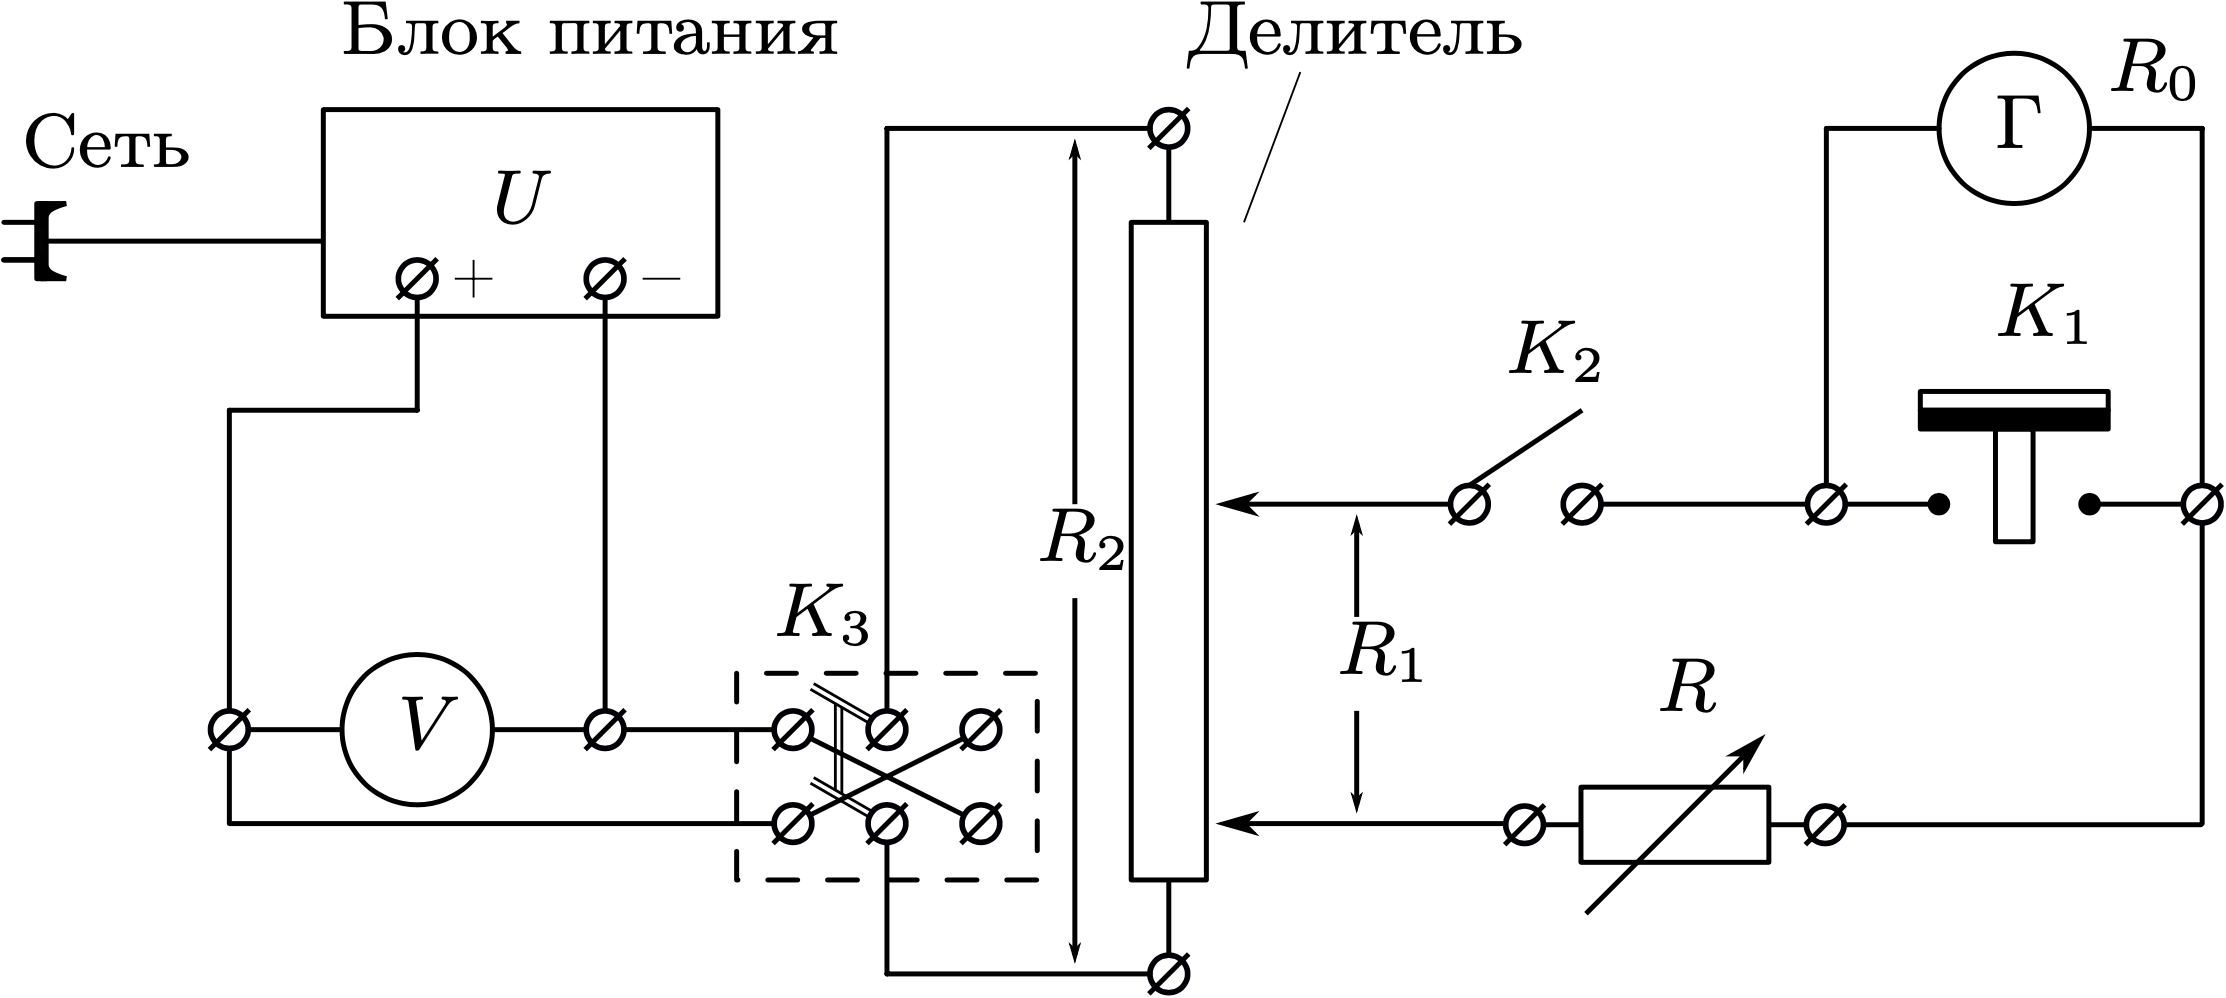
\includegraphics[width=0.8\linewidth]{images/scheme1.png}
        \caption{Схема установки для работы гальванометра в стационарном режиме}
        \label{pic1}
    \end{figure}
    
    При $R_1 \ll R, R_0, R_2$ сила тока, протекающего через гальванометр, может быть вычислена как
    \begin{equation}
        I = \frac{R_1}{R_2} \frac{U_0}{R + R_0},
        \label{eq1}
    \end{equation}
    где $U_0$ — показания вольтметра, $R_1/R_2$ — положение делителя, $R$ — сопротивление магазина, $R_0$ — внутреннее сопротивление гальванометра.
    
    Угол отклонения рамки от положения равновесия измеряется с помощью осветителя, зеркальца, укреплённого на рамке, и шкалы, на которую отбрасывается луч света от зеркальца. Координата $x$ светового пятна на шкале связана с углом $\varphi$ отклонения рамки формулой
    \begin{equation}
        x = a \text{ } \mathrm{arctg}(2 \varphi),
    \end{equation}
    где $a$ — расстояние от шкалы до зеркальца. При малых углах можно считать, что $\varphi = x/2a$. Динамическую постоянную
    \begin{equation}
        C_I = \frac{I}{\varphi} = \frac{2aI}{x},
        \label{eq2}
    \end{equation}
    как правило, выражают в единицах $\left[\frac{\text{А}}{\text{мм}/\text{м}}\right]$ (ток $I$ измеряется в амперах, $x$ – в миллиметрах, $a$ – в метрах). \\
    
    \noindent {\bf Б. Определение критического сопротивления гальванометра} \vspace{0.1cm}
    
    Критическим сопротивлением баллистического гальванометра называется сопротивление его электрической цепи $R_{кр}$, при котором после начального толчка подвижная система почти экспоненциально возвращается к нулю. На практике критический режим, требующий строгого выполнения условия $\gamma = \omega_0$, не может быть точно реализован и имеет значение как пограничный между режимом затухающих колебаний ($\gamma < \omega_0$) и режимом апериодического затухания ($\gamma > \omega_0$).
    
    Измерение критического сопротивления гальванометра можно выполнить с помощью той же схемы (рис. \ref{pic1}).
    
    При больших $R$ свободное движение рамки имеет колебательный характер. С уменьшением $R$ затухание увеличивается, и колебательный режим переходит в апериодический.

    В качестве характеристики процесса затухания колебаний рамки гальванометра воспользуемся представленным формулой логарифмическим декрементом затухания:
    \begin{equation}
        \Theta = \gamma T_1 = \mathrm{ln} \frac{x_n}{x_{n+1}},
        \label{eq3}
    \end{equation}
    где $x_n$ и $x_{n+1}$ — два последовательные отклонения колеблющейся величины в одну сторону. Измеряя зависимость $\Theta(R)$ логарифмического декремента затухания от сопротивления внешней цепи $R$, можно найти критическое сопротивление $R_{кр}$
    \begin{equation}
        R_{кр} = \frac{R + R_0}{\sqrt{\left( \frac{2 \pi}{\Theta} \right)^2 + 1}} - R_0,
        \label{eq4}
    \end{equation}
    или
    \begin{equation}
        \sqrt{\frac{4 \pi^2}{\Theta^2} + 1} = \frac{R + R_0}{R_{кр} + R_0}.
        \label{eq5}
    \end{equation} \\
    
    \noindent {\bf В. Определение баллистической постоянной и критического сопротивления гальванометра, работающего в баллистическом режиме} \vspace{0.1cm}
    
    Для изучения работы гальванометра в режиме измерения заряда (в баллистическом режиме), используется схема, представленная на рис. \ref{pic2}.
    
    Система ключей устроена так, что нормально ключ $K_2$ замкнут, а ключи $K_3$ и $K_4$ разомкнуты. При нажатии на кнопку $K_0$ сначала размыкается ключ $K_2$, затем замыкается $K_3$ и через некоторое время — $K_4$. При нормальном положении кнопки $K_0$ конденсатор $C$ заряжается до напряжения $U_C$ и получает заряд $q$:
    \begin{equation}
        U_C = \frac{R_1}{R_2} U_0, \hspace{1.5cm} q = C U_C = \frac{R_1}{R_2} U_0 C.
    \end{equation}
    При нажатии на ключ $K_0$ конденсатор отключается от источника постоянного напряжения (размыкается ключ $K_2$) и подключается к гальванометру (замыкается ключ $K_3$).
    
    \begin{figure}[ht]
        \centering
        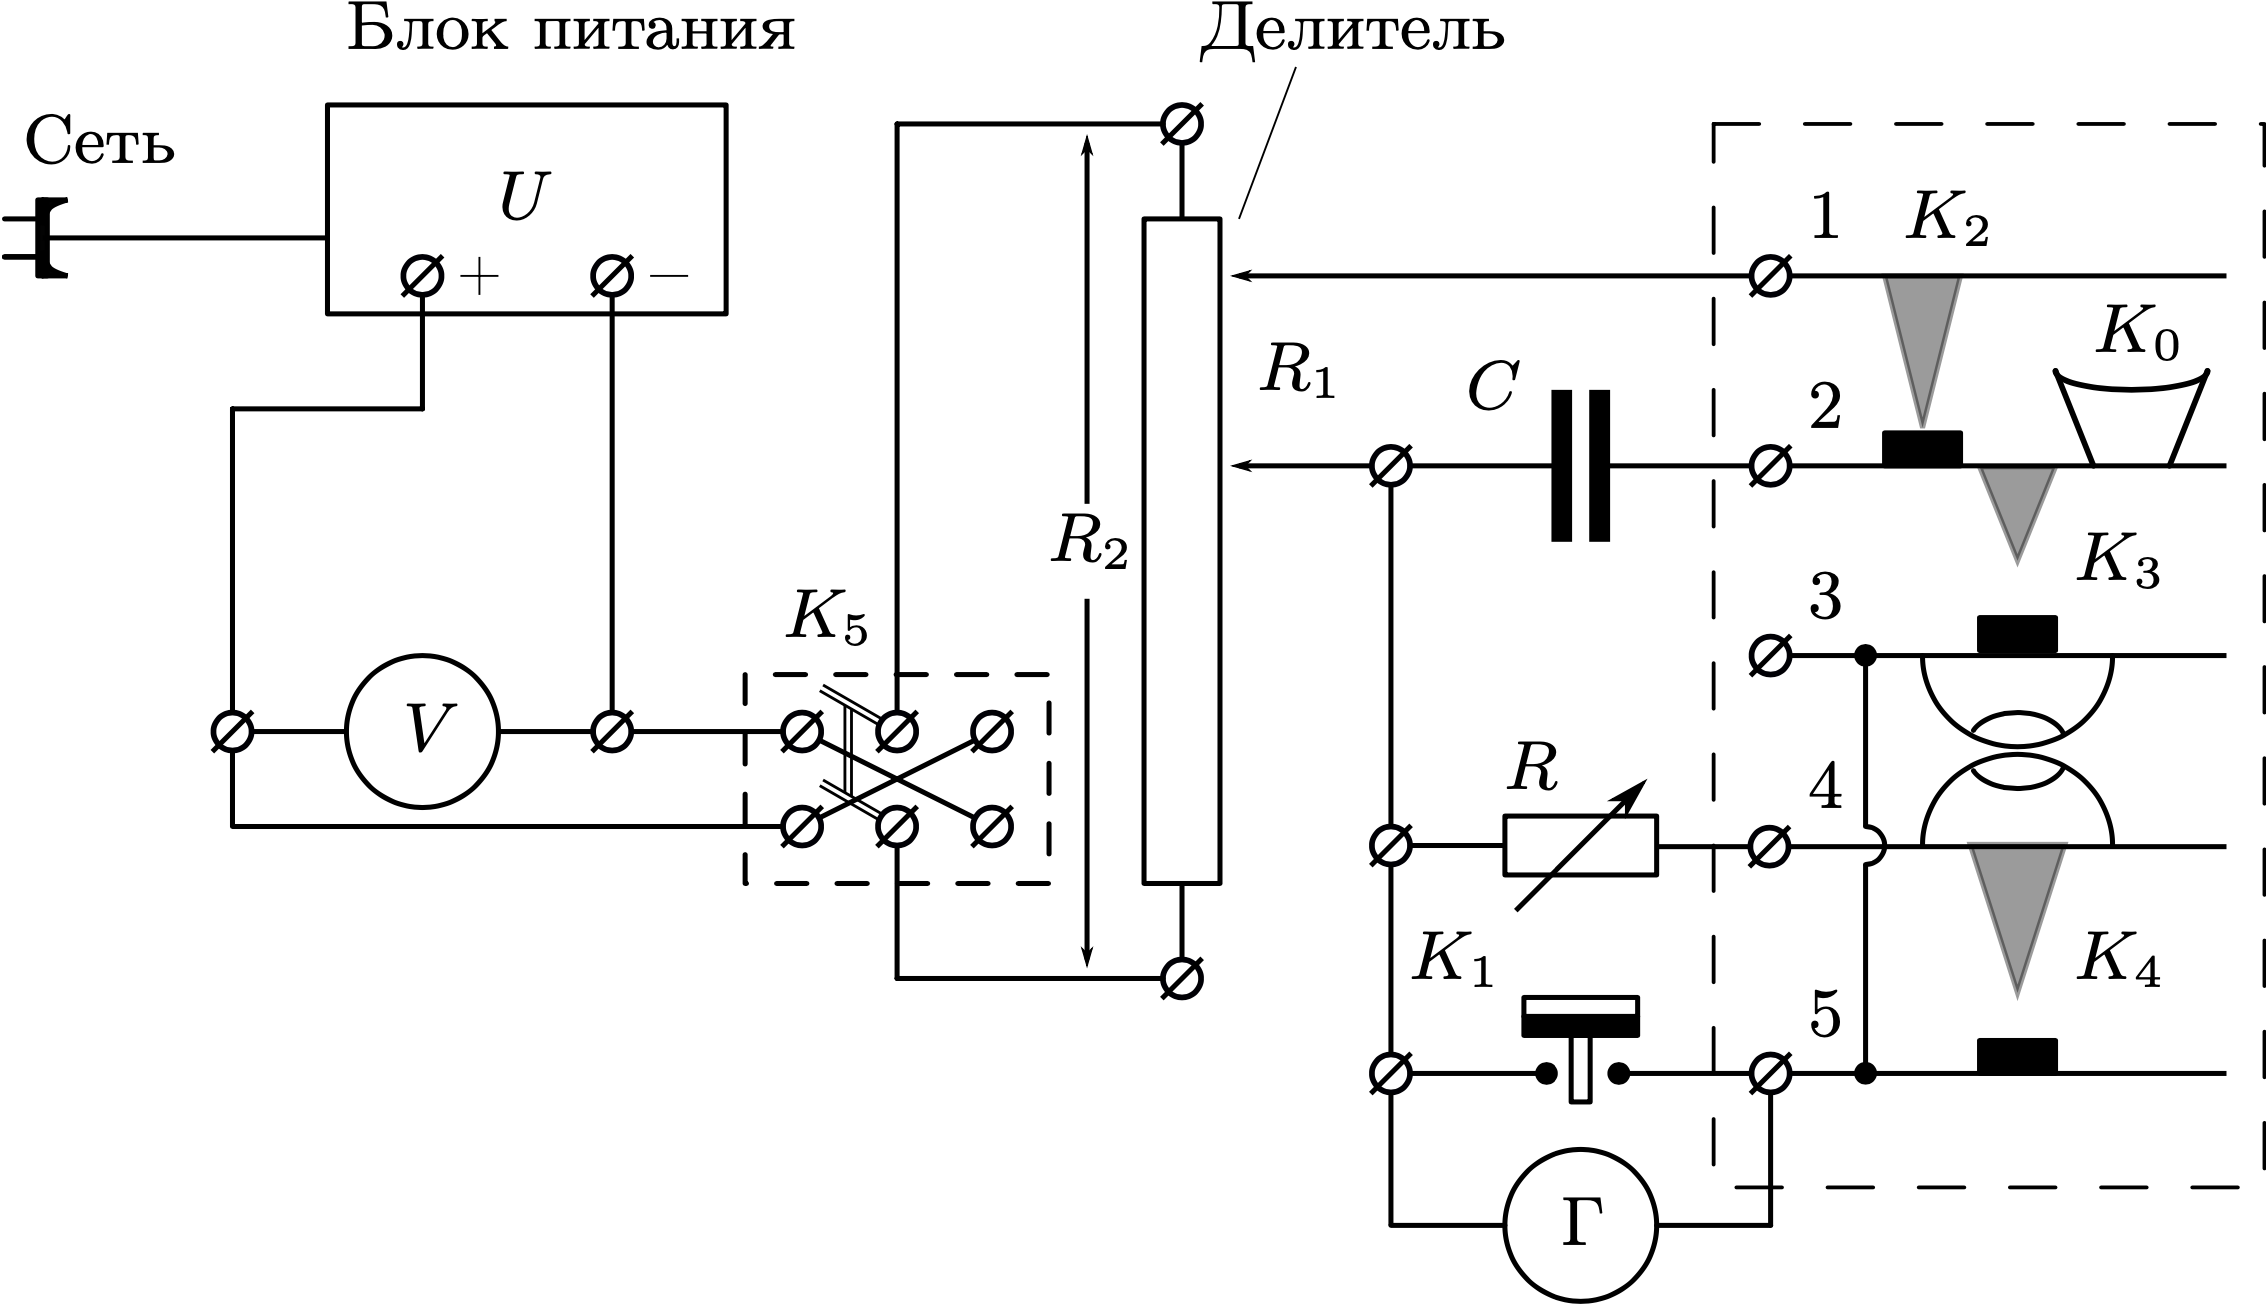
\includegraphics[width=0.8\linewidth]{images/scheme2.png}
        \caption{Схема установки для определения баллистической постоянной}
        \label{pic2}
    \end{figure}
    
    Ёмкость конденсатора выбрана так, что к моменту замыкания ключа $K_4$ весь заряд успевает пройти через гальванометр, и рамка получает начальную скорость $\dot{\varphi}(\tau)$. При этом можно считать, что отклонение рамки, происходящее за время, протекающее между замыканием ключей $K_3$ и $K_4$, равно нулю.
    
    Первый отброс зайчика $\varphi_{max}$ после нажатия на кнопку $K_0$ зависит от сопротивления внешней цепи, подключённой к гальванометру. Для определения $R_{кр}$ используется то обстоятельство, что в критическом режиме максимальное отклонение зайчика в $e$ раз меньше, чем у гальванометра без затухания.
    
    Следует помнить, что наблюдать колебания рамки при полном отсутствии затухания, конечно, невозможно, так как даже при разомкнутой внешней цепи ($R = \infty$) остаётся трение в подвеске и трение рамки о воздух. Величину максимального отклонения рамки гальванометра без затухания $\varphi^{св}_{max}$ можно, однако, рассчитать, если при разомкнутой цепи max измерить реальное максимальное отклонение рамки $\varphi_0$ и логарифмический декремент затухания $\Theta_0$ (при $R = \infty$ величина $\Theta_0$ определяется только внутренним трением в рамке). Из уравнений движения рамки при $\gamma \ll \omega_0$ вытекают равенства
    \begin{equation}
        \varphi_0 = \varphi(T_1/4) = \varphi^{св}_{max} e^{-\Theta_0/4},
    \end{equation}
    так что максимальное отклонение рамки гальванометра без затухания
    \begin{equation}
        \varphi^{св}_{max} = \varphi_0 e^{\Theta_0/4} \approx \varphi_0 \left( 1 + \frac{\Theta_0}{4} \right).
        \label{eq6}
    \end{equation}
    
    Баллистическая постоянная гальванометра $C^{кр}_q$ $\left[ \frac{\text{Кл}}{\text{мм}/\text{м}} \right]$ определяется при критическом сопротивлении ($R = R_{кр}$):
    \begin{equation}
        C^{кр}_q = \frac{q}{\varphi^{кр}_{max}} = 2a \frac{R_1}{R_2} \frac{CU_0}{x^{кр}_{max}},
        \label{eq7}
    \end{equation}
    где $x^{кр}_{max}$ – величина первого отброса в критическом режиме, выраженная в делениях шкалы (мм), $a$ – расстояние от зеркальца до шкалы, выраженное в метрах, произведение $CU_0$ – заряд, выраженный в кулонах.
    
    \newpage
    
    \begin{flushleft}
        {\Large {\bf Ход работы/Обработка результатов эксперимента}}
    \end{flushleft}
    
    \begin{enumerate}
    
        
        \item[1.] Подготовим к работе приборы, настроем гальванометр. Установим делитель напряжения на небольшое входное напряжение: $\frac{R_1}{R_2} = \frac{1}{2000}$. Соберём электрическую схему согласно рис. \ref{pic1}. Запишем также величину $R_2$, расстояние от шкалы до зеркальца гальванометра и внутреннее сопротивление гальванометра $R_0$, указанное на установке: $R_2 = 10 \text{ кОм}$; $a = 136,8 \text{ см}$; $R_0 = 610 \text{ Ом}$.
        
        Измерим зависимость отклонения зайчика $x$ от сопротивления магазина $R$, увеличивая сопротивление магазина, но не меняя делителя. По полученным данным рассчитаем токи $I$ через гальванометр по формуле \eqref{eq1} и построем график $I(x)$. Результаты будем заносить в табл. \ref{table1}, а график изобразим на рис. \ref{pic3}.
        
        \begin{table}[ht]
            \centering
            \begin{tabular}{|c||c|c|c|c|c|c|c|c|c|c|}
                \hline
                $R$, $\text{кОм}$ & 50 & 40 & 30 & 20 & 15 & 10 & 8 & 6 & 5 & 4 \\
                \hline
                $x$, $\text{мм}$ & 0 & 3 & 8 & 13 & 28 & 47 & 62 & 84 & 101 & 125 \\
                \hline
                $I$, $\text{нА}$ & 12,45 & 15,51 & 20,58 & 30,57 & 40,36 & 59,38 & 73,17 & 95,31 & 112,30 & 136,66 \\
                \hline
            \end{tabular}
            \caption{Зависимость отклонения зайчика от сопротивления, постоянный ток}
            \label{table1}
        \end{table}
        
        \begin{figure}[ht]
            \centering
            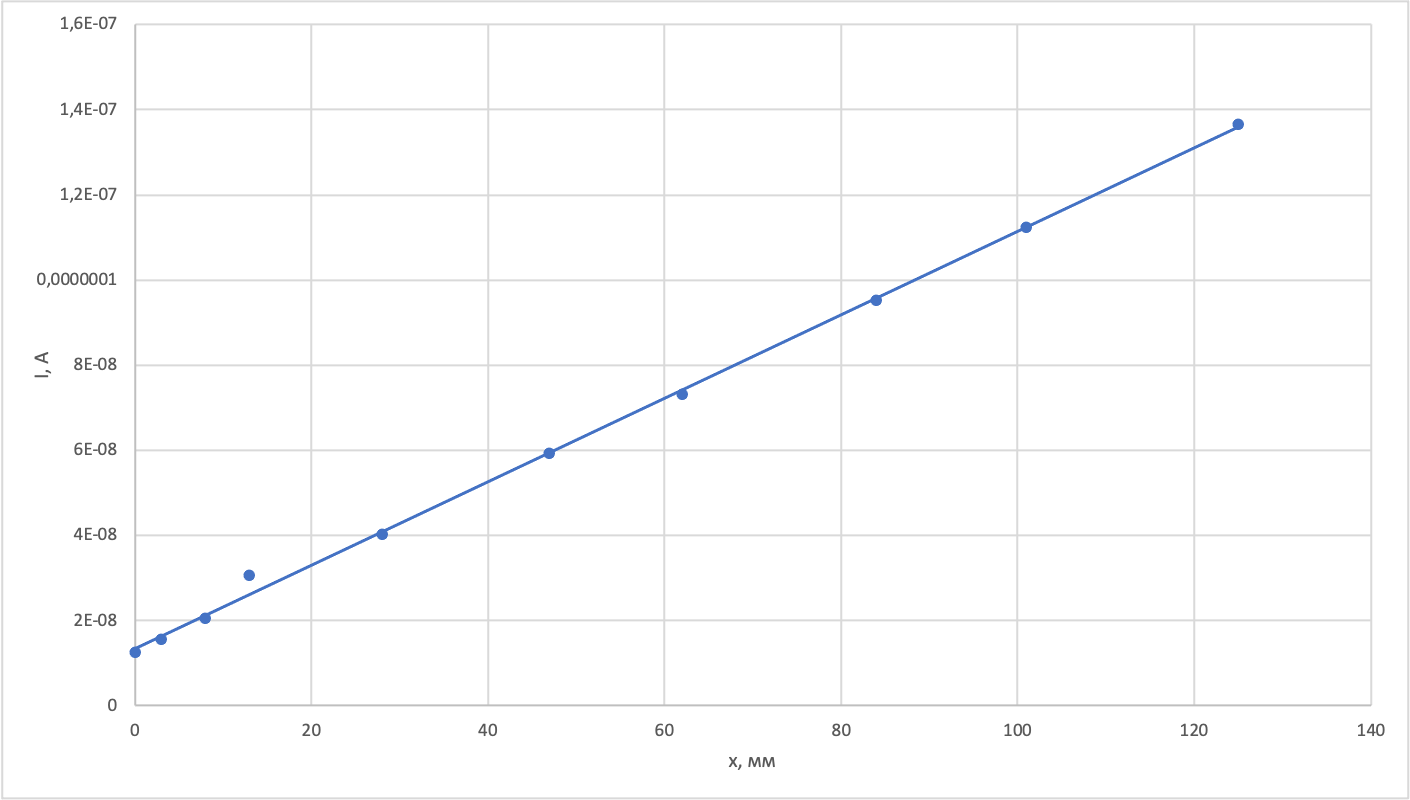
\includegraphics[width=0.9\linewidth]{images/I(x).png}
            \caption{График зависимости $I = f(x)$}
            \label{pic3}
        \end{figure}
        
        Пользуясь наклоном графика на рис. \ref{pic3}, рассчитаем динамическую постоянную $C_I$ гальванометра по формуле \eqref{eq2}. Получим результат:
        \begin{equation}
            C_I = (2,68 \pm 0,01) \cdot 10^{-9} \left[ \frac{\text{А}}{\text{мм}/\text{м}} \right]
        \end{equation}
        Рассчитаем также чувствительность гальванометра к току:
        \begin{equation}
            S_I = \frac{1}{C_I} = (3,73 \pm 0,12) \cdot 10^8 \left[ \frac{\text{мм}/\text{м}}{\text{А}} \right].
        \end{equation}
        
        
        \item[2.] Установим такое значение $R$, при котором зайчик отклоняется почти на всю шкалу: $R = 2 \text{ кОм}$. Разомкнём ключ $K_2$ и понаблюдаем за свободными колебаниями рамки. Измерим два последовательных отклонения зайчика в одну сторону для расчёта логарифмического декремента затухания $\Theta_0$ разомкнутого гальванометра. Получим результаты:
        \begin{equation}
            x_1 = 192 \text{ мм}, \hspace{2.5cm} x_2 = 160 \text{ мм}.
        \end{equation}
        Также приближённо измерим период $T_0$ свободных колебаний рамки. Получим:
        \begin{equation}
            T_0 = 3,35 \text{ с}.
        \end{equation}
        
        Пользуясь данными, полученными нами ранее, по формуле \eqref{eq3} рассчитаем логарифмический декремент затухания разомкнутого гальванометра. Получим:
        \begin{equation}
            \Theta_0 = (1,82 \pm 0,08) \cdot 10^{-1}.
        \end{equation}
        
        
        \item[3.] Снова замкнём ключ $K_2$ и убедимся, что зайчик находится на краю шкалы. Разомкнём ключ $K_3$. Теперь подберём наибольшее сопротивление магазина $R$, при котором при замыкании ключа $K_3$ зайчик не переходит за нулевое значение. Это сопротивление близко к критическому: $R_{кр} \approx 4,5 \text{ кОм}$.
        
        Установим сопротивление магазина $R \approx 3 R_{кр}$ и подберём делитель так, чтобы в стационарном режиме зайчик отклонялся почти на всю шкалу: $\frac{R_1}{R_2} = \frac{1}{300}$. Рассчитаем декремент затухания $\Theta$, измеряя дво последовательных отклонения зайчика в одну сторону после размыкания ключа $K_3$. Повторим измерения декремента затухания для других значений $R$, постепенно увеличивая сопротивление магазина до $10 R_{кр}$. Результаты будем заносить в табл. \ref{table2}.
        
        \begin{table}[ht]
            \centering
            \begin{tabular}{|c||c|c|c|c|c|c|c|c|c|c|}
                \hline
                $R$, $\text{кОм}$ & 13,50 & 18,00 & 20,25 & 22,50 & 24,75 & 27,00 & 31,50 & 36,00 & 40,50 & 45,00 \\
                \hline
                $x_1$, $\text{мм}$ & 55 & 64 & 62 & 62 & 62 & 62 & 58 & 65 & 54 & 49 \\
                \hline
                $x_2$, $\text{мм}$ & 3 & 7 & 9 & 11 & 13 & 14 & 15 & 20 & 19 & 19 \\
                \hline
                $\Theta$ & 2,91 & 2,21 & 1,93 & 1,73 & 1,56 & 1,49 & 1,35 & 1,18 & 1,04 & 0,95 \\
                \hline
            \end{tabular}
            \caption{Зависимость декремента затухания от сопротивления магазина}
            \label{table2}
        \end{table}
        
        Пользуясь данными табл. \ref{table2}, построим график $1/\Theta^2 = f[(R + R_0)^2]$ и по формуле \eqref{eq5} рассчитаем значение критического сопротивления $R_0$ (в области малых $R$). График приведём на рис. \ref{pic4}.
        
        Рассчитаем значение $R_0$, пользуясь первыми пяти точками. В итоге получим:
        \begin{equation}
            R_0 = 5580 \pm 123 \text{ Ом}.
        \end{equation}
        
        
        \item[4.] Перейдём к работе гальванометра в баллистическом режиме. Соберём схему согласно рис. \ref{pic2}. Запишем параметры и показания вспомогательных приборов: $C = 2 \text{ мкФ}$; $U_0 = 1,26 \text{ В}$. Установим на магазине сопротивление $R = 50 \text{ кОм}$. Разомкнём цепь $R$, отсоединив одну из клемм от магазина. Подберём делитель так, чтобы при замыкании ключа $K_0$ первый отброс $l_{max}$ соотвествовал отклонению зайчика почти на всю шкалу: $R_1/R_2 = 1/20$. Запишем значение первого отброса для свободных колебаний: $l_0 = 237 \text{ мм}$. Вновь подключим магазин $R$. Получим зависимость первого отброса от величины $R$. Будем уменьшать $R$ до тех пор, пока первый отброс не уменьшится до $1/3 – 1/4$ от максимальной величины. Результаты будем заносить в табл. \ref{table3}.
        
        Теперь построим график зависимости $l_{max} = f[(R + R_0)^{-1}]$. График представим на рис. \ref{pic5}.
        
        \newpage
        
        \begin{figure}[ht]
            \centering
            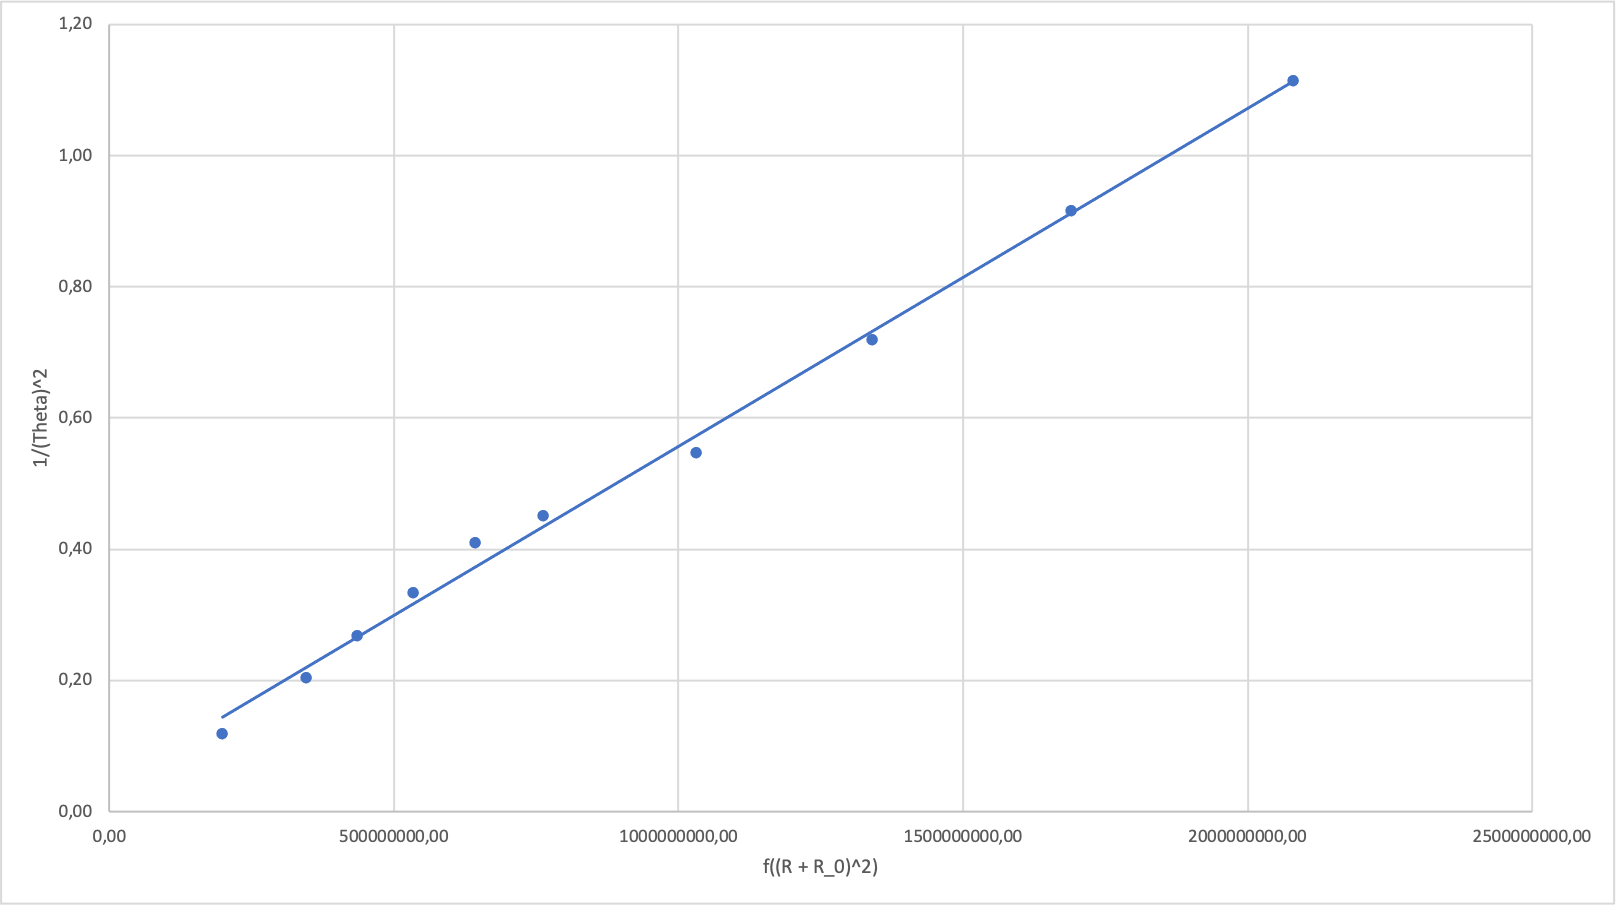
\includegraphics[width=0.9\linewidth]{images/graph2.png}
            \caption{График зависимости $1/\Theta^2 = f[(R + R_0)^2]$}
            \label{pic4}
        \end{figure}
        
        \begin{table}[ht]
            \centering
            \begin{tabular}{|c||c|c|c|c|c|c|c|c|c|c|}
                \hline
                $R$, $\text{кОм}$ & 50 & 40 & 35 & 30 & 25 & 20 & 15 & 10 & 5 & 2,5 \\
                \hline
                $l_{max}$, $\text{мм}$ & 163 & 157 & 155 & 148 & 149 & 138 & 120 & 96 & 61 & 40 \\
                \hline
            \end{tabular}
            \caption{Зависимость первого отброса от сопротивления магазина}
            \label{table3}
        \end{table}
        
        \begin{figure}[h!]
            \centering
            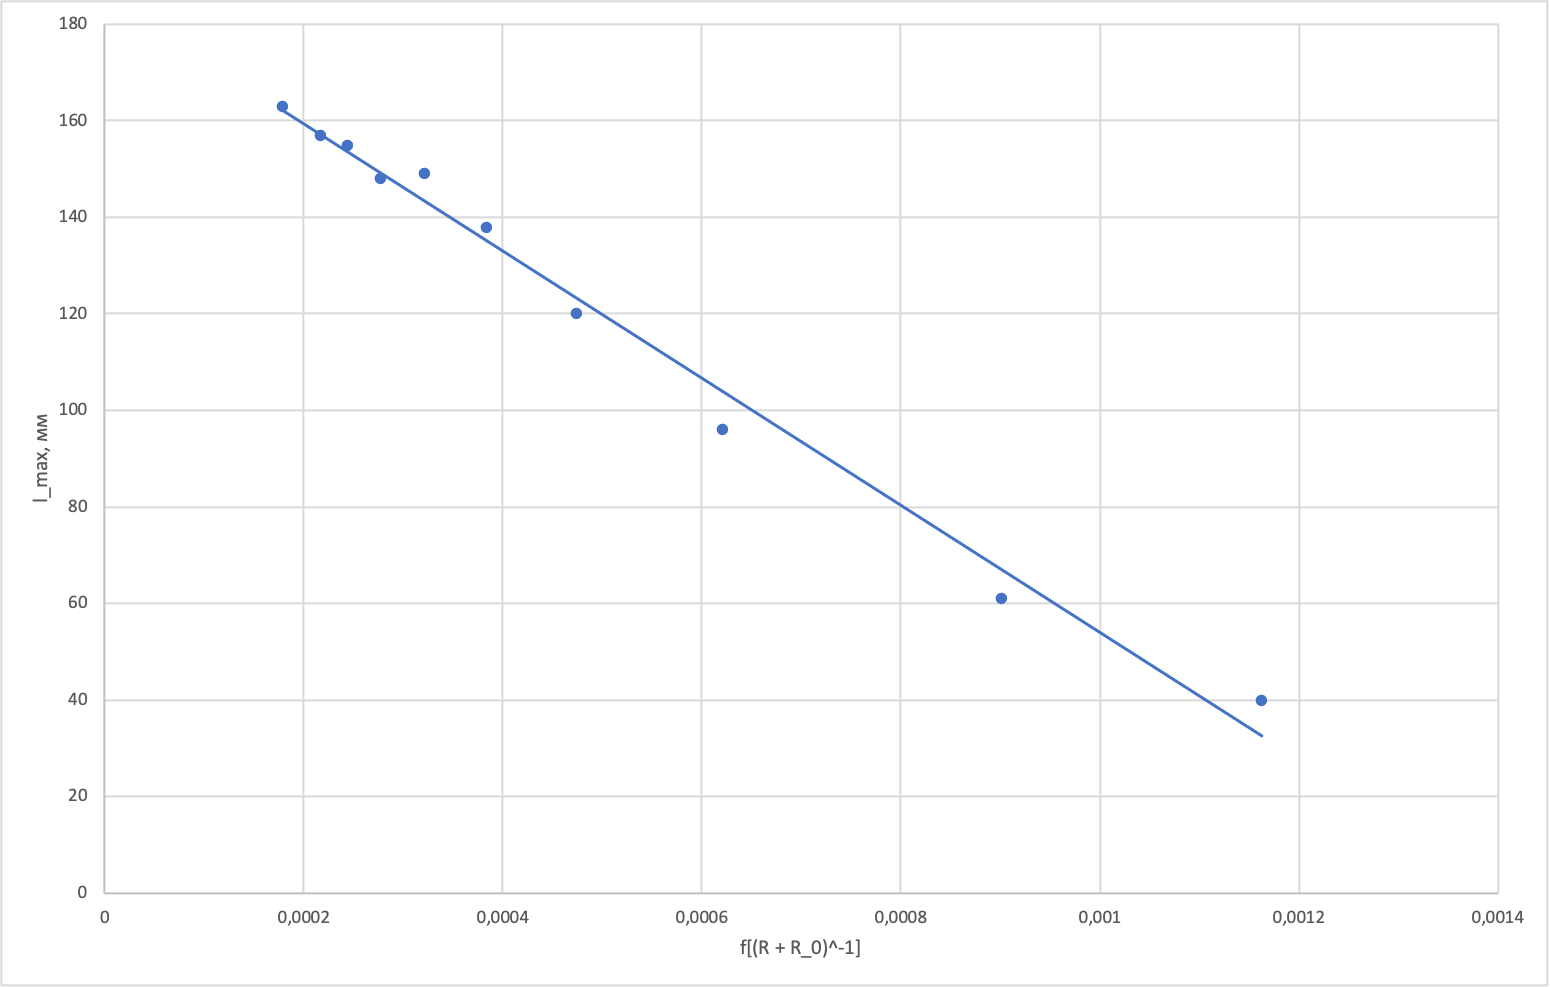
\includegraphics[width=0.9\linewidth]{images/graph3.png}
            \caption{График зависимости $l_{max} = f[(R + R_0)^{-1}]$}
            \label{pic5}
        \end{figure}
        
        \newpage
        
        Определим по рис. \ref{pic5} критическое сопротивление гальванометра:
        \begin{equation}
            R_{кр} \approx 723 \text{ Ом}.
        \end{equation}
        
        \item[5.] Рассчитаем баллистическую постоянную в критическом режиме $C^{кр}_q$ по формуле \eqref{eq7}. Получим:
        \begin{equation}
            C^{кр}_q = (4,00 \pm 0,23) \cdot 10^{-9} \left[ \frac{Кл}{мм/м} \right].
        \end{equation}
        
        
        \item[6.] Сравним время релаксации $t = R_0 C$ и период свободных колебаний гальванометра $T_0$:
        \begin{equation}
            t = 0,00122 \text{ с} \ll T_0 = 3,35 \text{ с},
        \end{equation}
        время релаксации сильно меньше периода свободных колебаний. Значит эксперимент и данные полученные нами корректны.
        
        
    \end{enumerate}
    
    \begin{flushleft}
        {\Large {\bf Вывод}}
    \end{flushleft}
    
    В ходе данной работы нами были получены динамическая постоянная и баллистическая постоянная гальванометра, а также тремя разными способами было получено значение критического сопротивления гальванометра. В конце обработки результатов была проверена корректность данного эксперимента и всех полученных результатов, путём сравнения времени релаксации и периода свободных колебаний гальванометра.
    
\end{document}